\vspace{-5mm}
\section{\uppercase{Design and Architecture}}
\label{sec:architecture}

% principles
\noindent Workflow and requirements described in the previous section have been received in a prototypal application serving as proof of concept. With the aim of maximize accessibility for surveyors, it is strongly web based and runs in all modern browsers. It is built using React by Facebook and an MVC design pattern with \emph{unidirectional data flow} \cite{redux}:  it ensures the best code maintainability and debuggability by centralizing access to the application state to a single controller.

\vspace{-3mm}\subsection{UI \& UX}\vspace{-3mm}

The web application presents itself as a simplified CAD,  the UI comprises three main areas of interaction: \emph{toolbar}, \emph{canvas} and \emph{sidebar}, as shown by Figures~\ref{fig:ui} and~\ref{fig:ui2}.

\begin{figure}[htbp] %  figure placement: here, top, bottom, or page
   \centering
   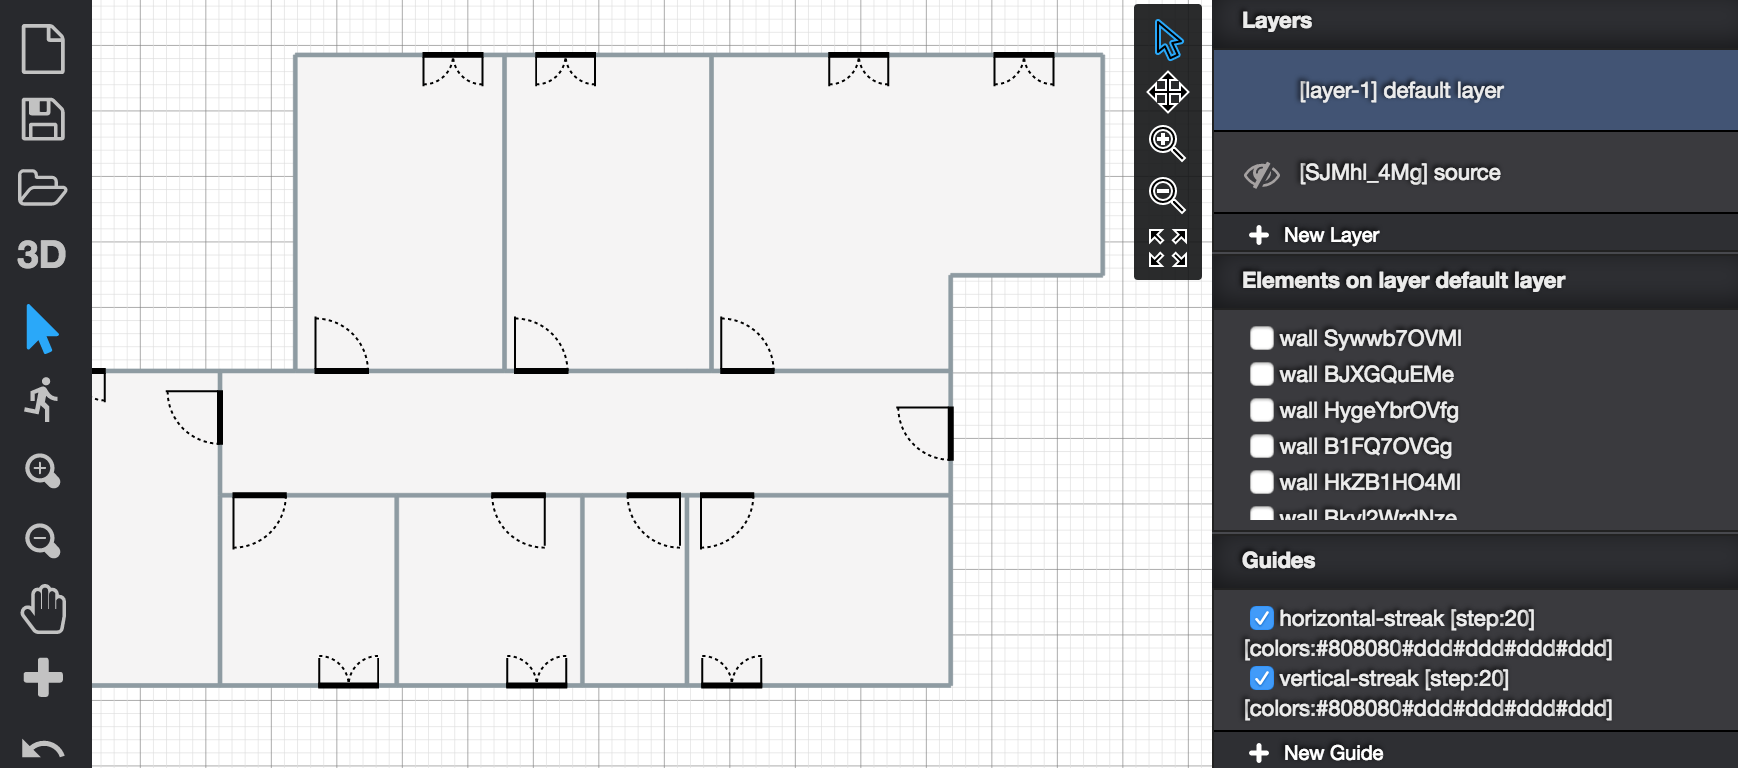
\includegraphics[width=1\linewidth]{images/2d}
   \label{fig:ui}
   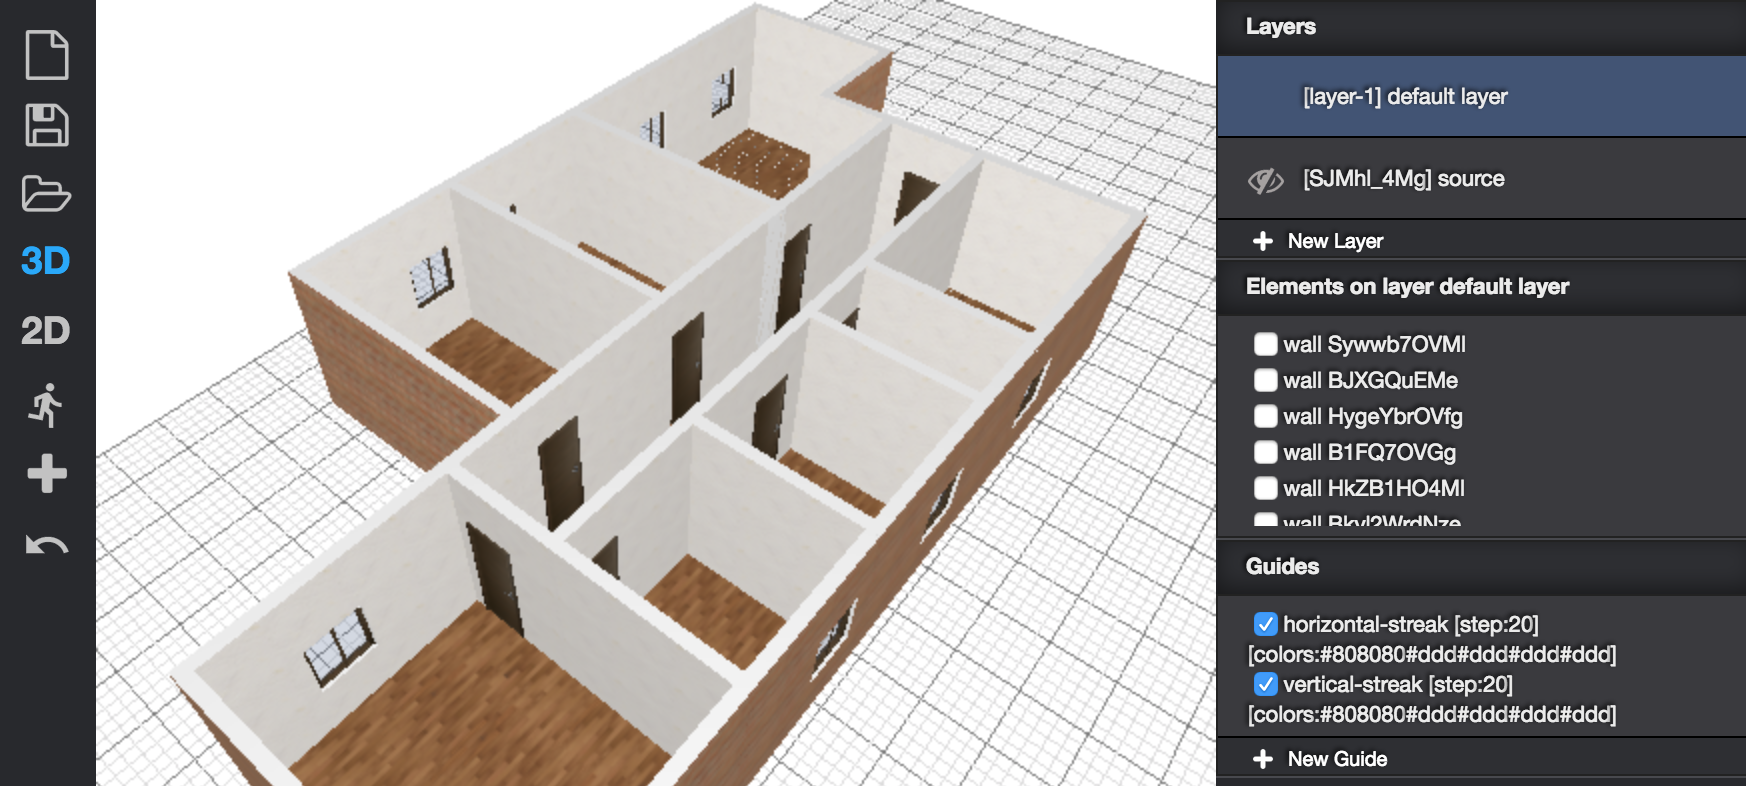
\includegraphics[width=1\linewidth]{images/3d}
   \caption{\emph{Metior} user interface: (a) 2D canvas; (b) 3D canvas}
   \label{fig:ui2}
\end{figure}

From the \emph{toolbar} the user can access functionalities related to: project life cycle ({\tt new}, {\tt save}, {\tt load}); project editing  ({\tt  show-catalog}); view/interaction mode switching ({\tt 2D}, {\tt  3D}); interaction mode changing ({\tt  selecting}, {\tt pan}, {\tt zoom}).


The \emph{canvas} is the area in which the user can interact with actual model data. It supports two different view and interaction modes. In~\emph{2D-mode} the model is displayed as a 2D projection from the top, and the interaction consists of element insertion, selection and editing (according to specific plugin interaction prototype, see~\ref{ssec:taxonomy}). In~\emph{3D-mode} a 3D model can be inspected and navigated, respectively via trackball or first-person interaction style, while object picking allows for element selection.

The \emph{sidebar} shows the properties of the currently selected element.
In the properties panel it is possible to view the description of the element, to add/remove metadata, and to modify any property. The latter is the interaction mode that allows the user to associate semantics annotations to every part of the model.

\vspace{-3mm}\subsection{Plugin-architecture}\vspace{-3mm}

\noindent The application has been designed to provide a small set of core interaction functionalities and to encapsulate the generation logic for architectural components (from the very basic to the most articulated) into specific plugins.

A \emph{plugin} is a software component that can be seamlessly integrated into the system in order to extends its capabilities.
In \emph{Metior}, a plugin represents an architectural element that extends the Building Information Model design.
Technically, a plugin represents a \emph{prototype} (namely a ``class'' in OOP) of a construction element that can be inserted (``instantiated'') into the \emph{canvas}, thus defining a new element, i.e. a new component of the model.

\vspace{-3mm}\paragraph{Plugin definition}

A plugin is described by the following eight properties: (1) a unique name; (2) a description; (3) a set of metadata; (4) the \emph{occupation type} (one among \emph{linear}, \emph{area} or \emph{volume}); (5) the \emph{placement type} (\emph{inside} or \emph{over}); (6) a set of specific properties mapping the semantic to associate to the plugin; (7) a \emph{generating function} that returns the 2D representation of the element in SVG format, to be used in the \emph{2D-mode}; (8) a \emph{generating function} that returns the 3D representation of the element in OBJ format, to be used in the \emph{3D-mode}.

\vspace{-3mm}\paragraph{Plugins taxonomy}\label{ssec:taxonomy}

\noindent The plugins can be organized according to the \emph{occupation type} and the \emph{placement type}. 

In the \emph{occupation type} three different kind of plugins can be identified: \emph{linear}, \emph{area} or \emph{volume} plugins.
The \emph{linear} ones extend in one dimension (unless a radial thickness) (e.g. hydraulic lines, electrical cables). The \emph{area} plugins extend in two dimensions (unless a linear thickness), (e.g. separation elements). They can be divided into \emph{horizontal area} (e.g. floor and ceil), and \emph{vertical area}, (e.g. walls). The \emph{volume} plugins extend in three dimensions. They can be \emph{fixed volume}, (e.g. a piece of furniture) and \emph{scalable volume}, that can be scaled (proportionally or not), (eg. pillars, staircases).

The \emph{occupation type} determines a different way to instantiate and to insert the plugins into the canvas.
In particular, in \emph{2D-mode}, \emph{linear} plugins are inserted drawing lines by mean of a drag\&drop interaction;
the \emph{area} plugins are inserted drawing the bounding-box of the element by mean of a drag\&drop interaction;
the \emph{volume} plugins are inserted picking the position of the element by mean of a point\&click interaction,
and adjusting their dimensions modifying the bounding-box by drag\&drop.

The \emph{placement type} determines if the element can be inserted into the canvas in a specific point occupied or not by other elements. In other words 
the {placement type} determines the relationship between a new instance of a plugin and instances of other plugins previously added to the model. The relationship can be of two kind: \emph{inside} or \emph{over}.
Plugins belonging to the \emph{inside} category can be added only inside other element (that can be \emph{linear}, \emph{area} or \emph{volume}); e.g., a ``window'' is a ``volume inside vertical area'' element,
while an ``hydraulic line'' is a ``linear inside horizontal area'' element.
Plugins of the \emph{over} category can be added only over other elements (of any type);
e.g., a ``pillar'' is a ``volume over horizontal area'' element,
while an ``electric panel'' is a ``volume over vertical area'' element.

In the design phase, an element that doesn't meet the placement constraints defined by the \emph{placement type} is notified by the system as a visual warning, showing its bounding-box in semi-transparent blinked red color.

\begin{figure}[htbp] %  figure placement: here, top, bottom, or page
   \centering

   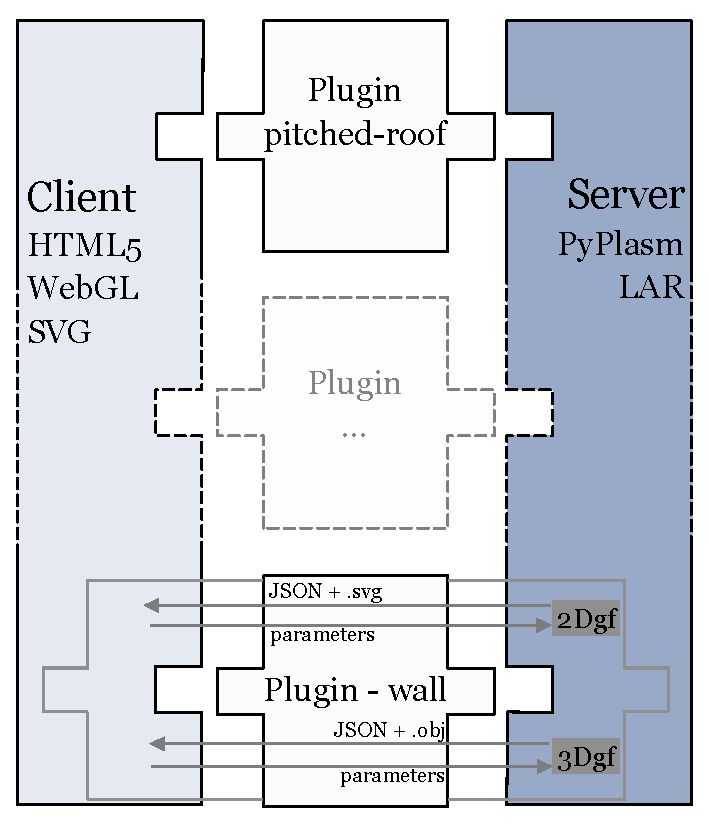
\includegraphics[width=0.6\linewidth]{images/architecture-h}

   \caption{Client/Server architecture for server-side model generation.}
   \label{fig:c-s-arch}
\end{figure}

\vspace{-3mm}\paragraph{Plugin specific properties}

\noindent Each plugin has a set of specific properties of the building elements it represents.
Each property is defined by a  \emph{name}, a \emph{type}, such as ``number'', ``text'', ``boolean'', or ``custom'', and by a \emph{value}.
According to its type, each property value can be inserted in different ways.
For example, a boolean property value is set through a checkbox, while a textual property is set through a text box.

The system is designed to accept custom kinds of property. A custom property is required to define the component of the UI that permit the user to insert its value.
For example, a ``color'' property can be introduced by defining a UI component composed by three text boxes (one for each RGB components), while a ``length'' property can be introduced by defining a UI component including a text box for the value and a drop-down menu for the unit of measure.

The specific properties of an element can be edited in the relative panel in the sidebar, once the element is selected in the canvas.

\vspace{-3mm}\subsection{Plugin Catalog}\vspace{-3mm}
\noindent It is pivotal to provide surveyors with a rich catalog of plugins, to cover all the basic as well as the most advanced modeling requirements. Table~\ref{tab:plugins-example} reports examples of plugins arranged according to the  taxonomy introduced in Section~\ref{ssec:taxonomy}.

\begin{table}[htbp]
\small
\centering
\caption{Plugin examples according to taxonomy}
\begin{tabular}{|
>{\columncolor[HTML]{EFEFEF}}l |l|l|}
\hline
{\color[HTML]{000000} } & \cellcolor[HTML]{EFEFEF}{\color[HTML]{000000} \footnotesize{\bf{inside}}} & \cellcolor[HTML]{EFEFEF}{\color[HTML]{000000} \footnotesize{\bf{over / free}}} \\ \hline
\footnotesize{\bf{linear}}      & \tt{pipe}             & \tt{electrical-conduit}  \\ \hline
\footnotesize{\bf{ver. area}}   & \tt{window, door}     & \tt{wall}                \\ \hline
\footnotesize{\bf{hor. area}}   & \tt{light-panel}      & \tt{ground, ceil}        \\ \hline
\footnotesize{\bf{volume}}      & \tt{pillar}           & \tt{staircase}           \\ \hline
\end{tabular}
\label{tab:plugins-example}
\end{table}


\vspace{-3mm}\subsection{Server-side models generation}\vspace{-3mm}

\noindent Both the 3D and 2D model generations have been designed as \emph{asynchronous}. The actual result of the invocation of a generating function is not the generated model itself, but rather a \emph{promise} of the expected result. Such a design choice is important since the computation for model generation may require some while. In the meantime the user must be able to interact with the interface, which in turn must remain responsive. Relying on this architecture, generation of the models can be easily delegated to a server (as shown in Figure~\ref{fig:c-s-arch}), thus relieving the client from the burden of onerous computations. The server exposes a REST-like HTTP-based JSON API to the client. The plugins span from the client to the server, since the 2D and 3D generating functions  defined by the plugin, with superclasses \emph{2Dgf} and \emph{3Dgf}, are actually executed on the server, as shown in Figure~\ref{fig:c-s-arch} .


\vspace{-1mm}\subsection{Plugin example}\vspace{-3mm}

In Figure~\ref{spiralstair} is shown the plugin used to generate a spiral concrete frame, where the steps are obtained by coded update of the polyhedral approximation of \texttt{larSolidHelicoid}, with parametric minor and major radiuses (\texttt{r} and \texttt{R}) and int number of \texttt{steps}. The \texttt{nturns} float is in radians.

\begin{figure}[h] %  figure placement: here, top, bottom, or page
   \centering
   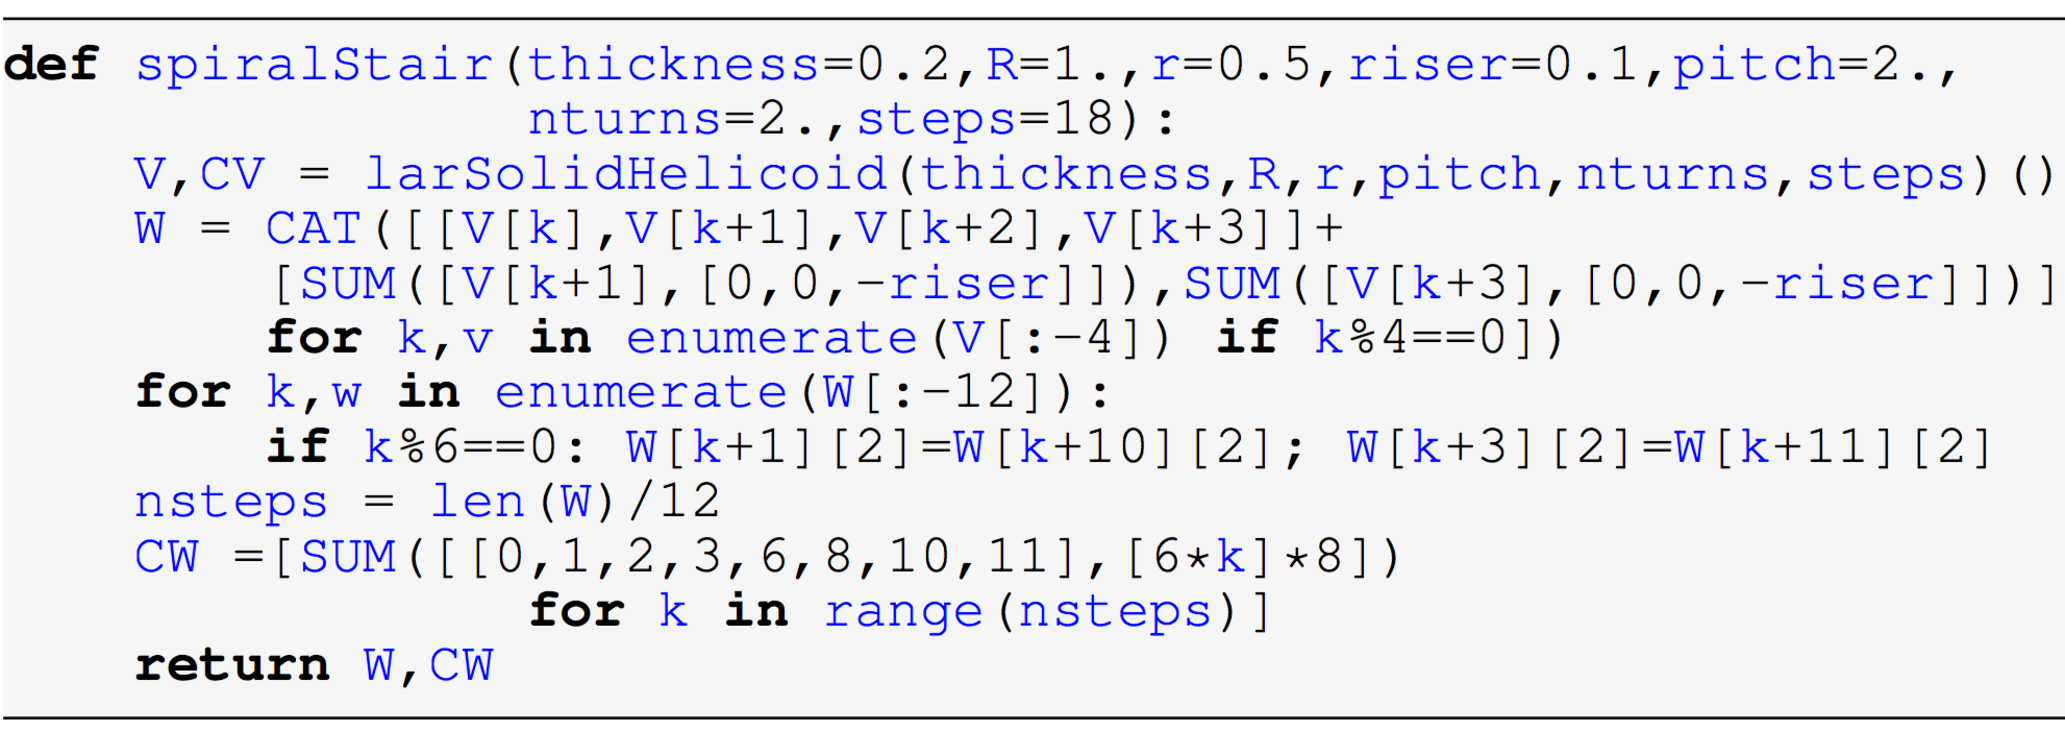
\includegraphics[width=\linewidth]{images/spiralstair}
   
   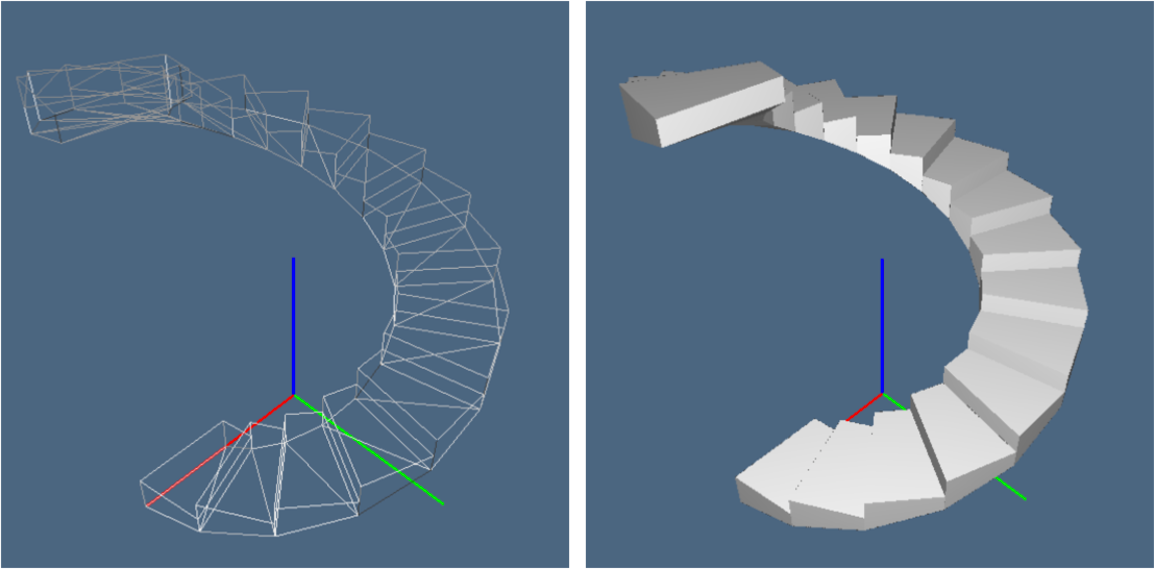
\includegraphics[width=\linewidth]{images/spiralstair2}
   \caption{(a) The generating function of a strongly parameterized \texttt{spiralStair}; (b) default \texttt{spiralStair}.}
   \label{spiralstair}
\end{figure}


